\section{Problem Setting}

\begin{frame}
	\begin{figure}[t]
		\centering
		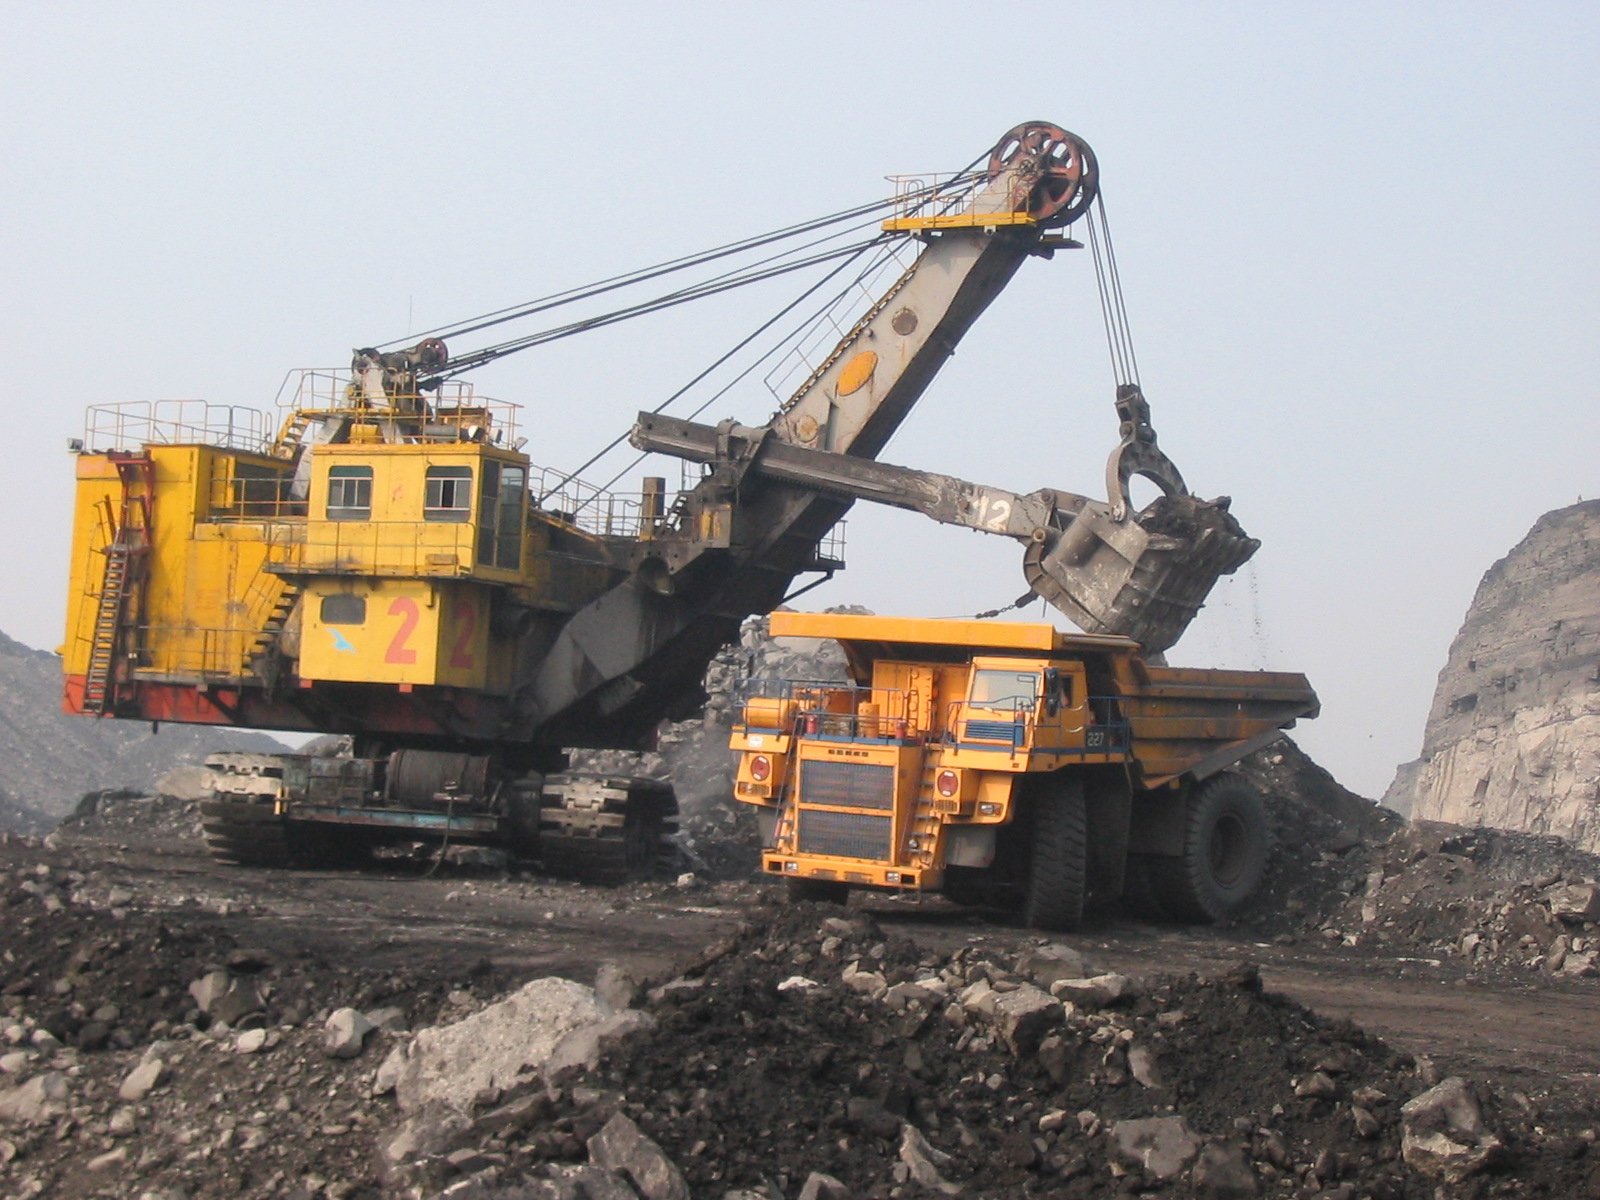
\includegraphics[width=.6\linewidth]{img/Excavator} \\
		\tiny{originally posted to Flickr by FAndrey at http://flickr.com/photos/43301444@N06/4141786255}
	\end{figure}

	\begin{itemize}
		\item{Goal: \textbf{optimization of model parameters}}
		\item{Models of technical system = physical properties + control properties}
	\end{itemize}
\end{frame}

\begin{frame}
	\frametitle{Problem Setting}
	\begin{figure}[bth]
		\centering
		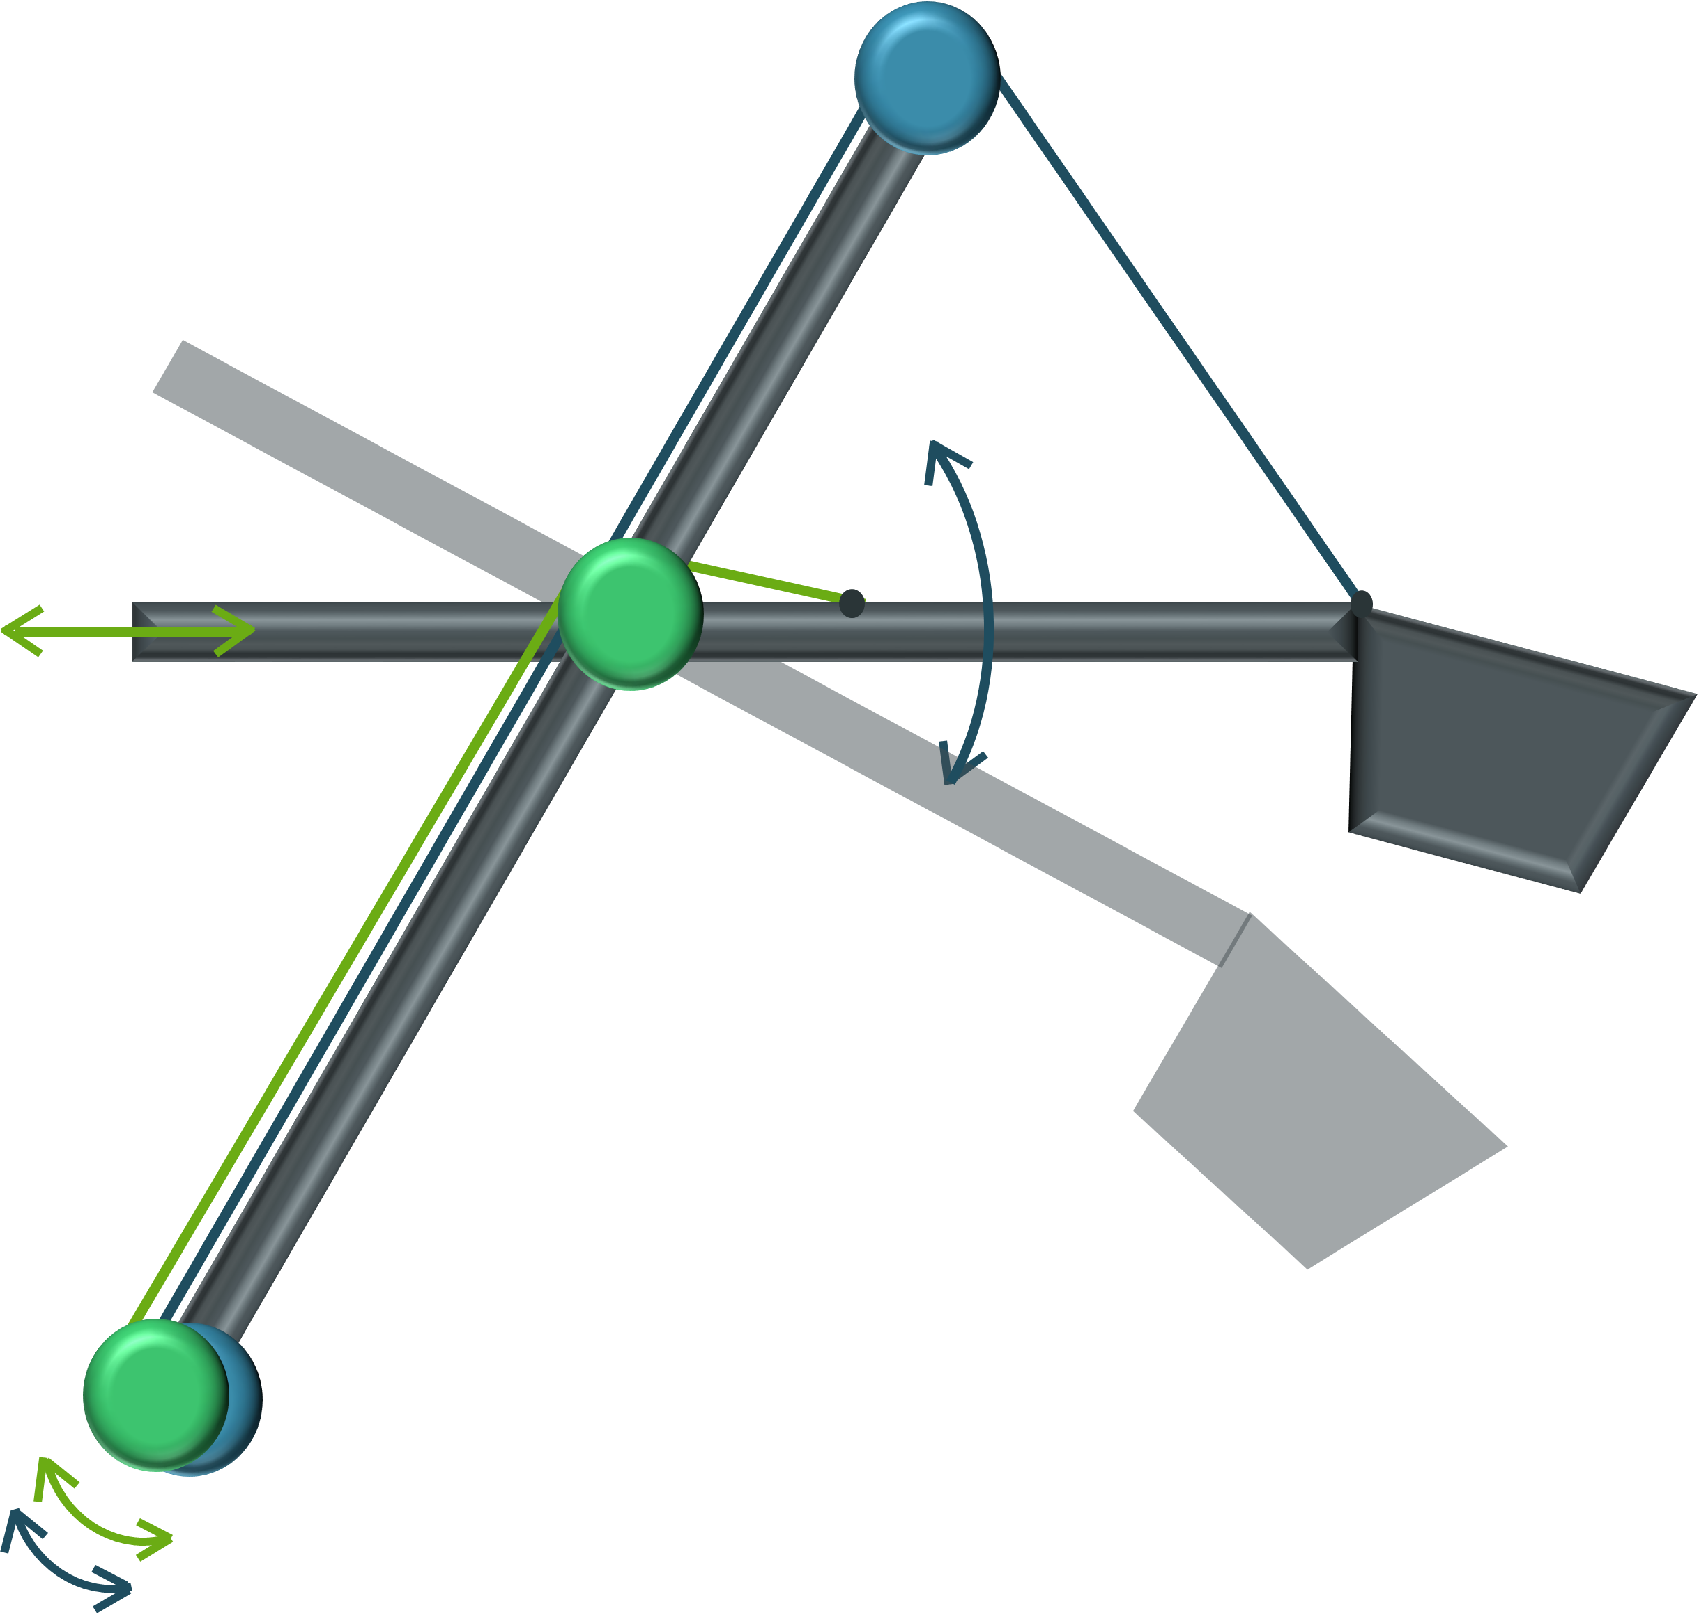
\includegraphics[width=0.4\linewidth]{img/Problem_1}
	\end{figure}
\end{frame}

\begin{frame}
	\frametitle{Problem Setting}
	\begin{figure}[bth]
		\centering
		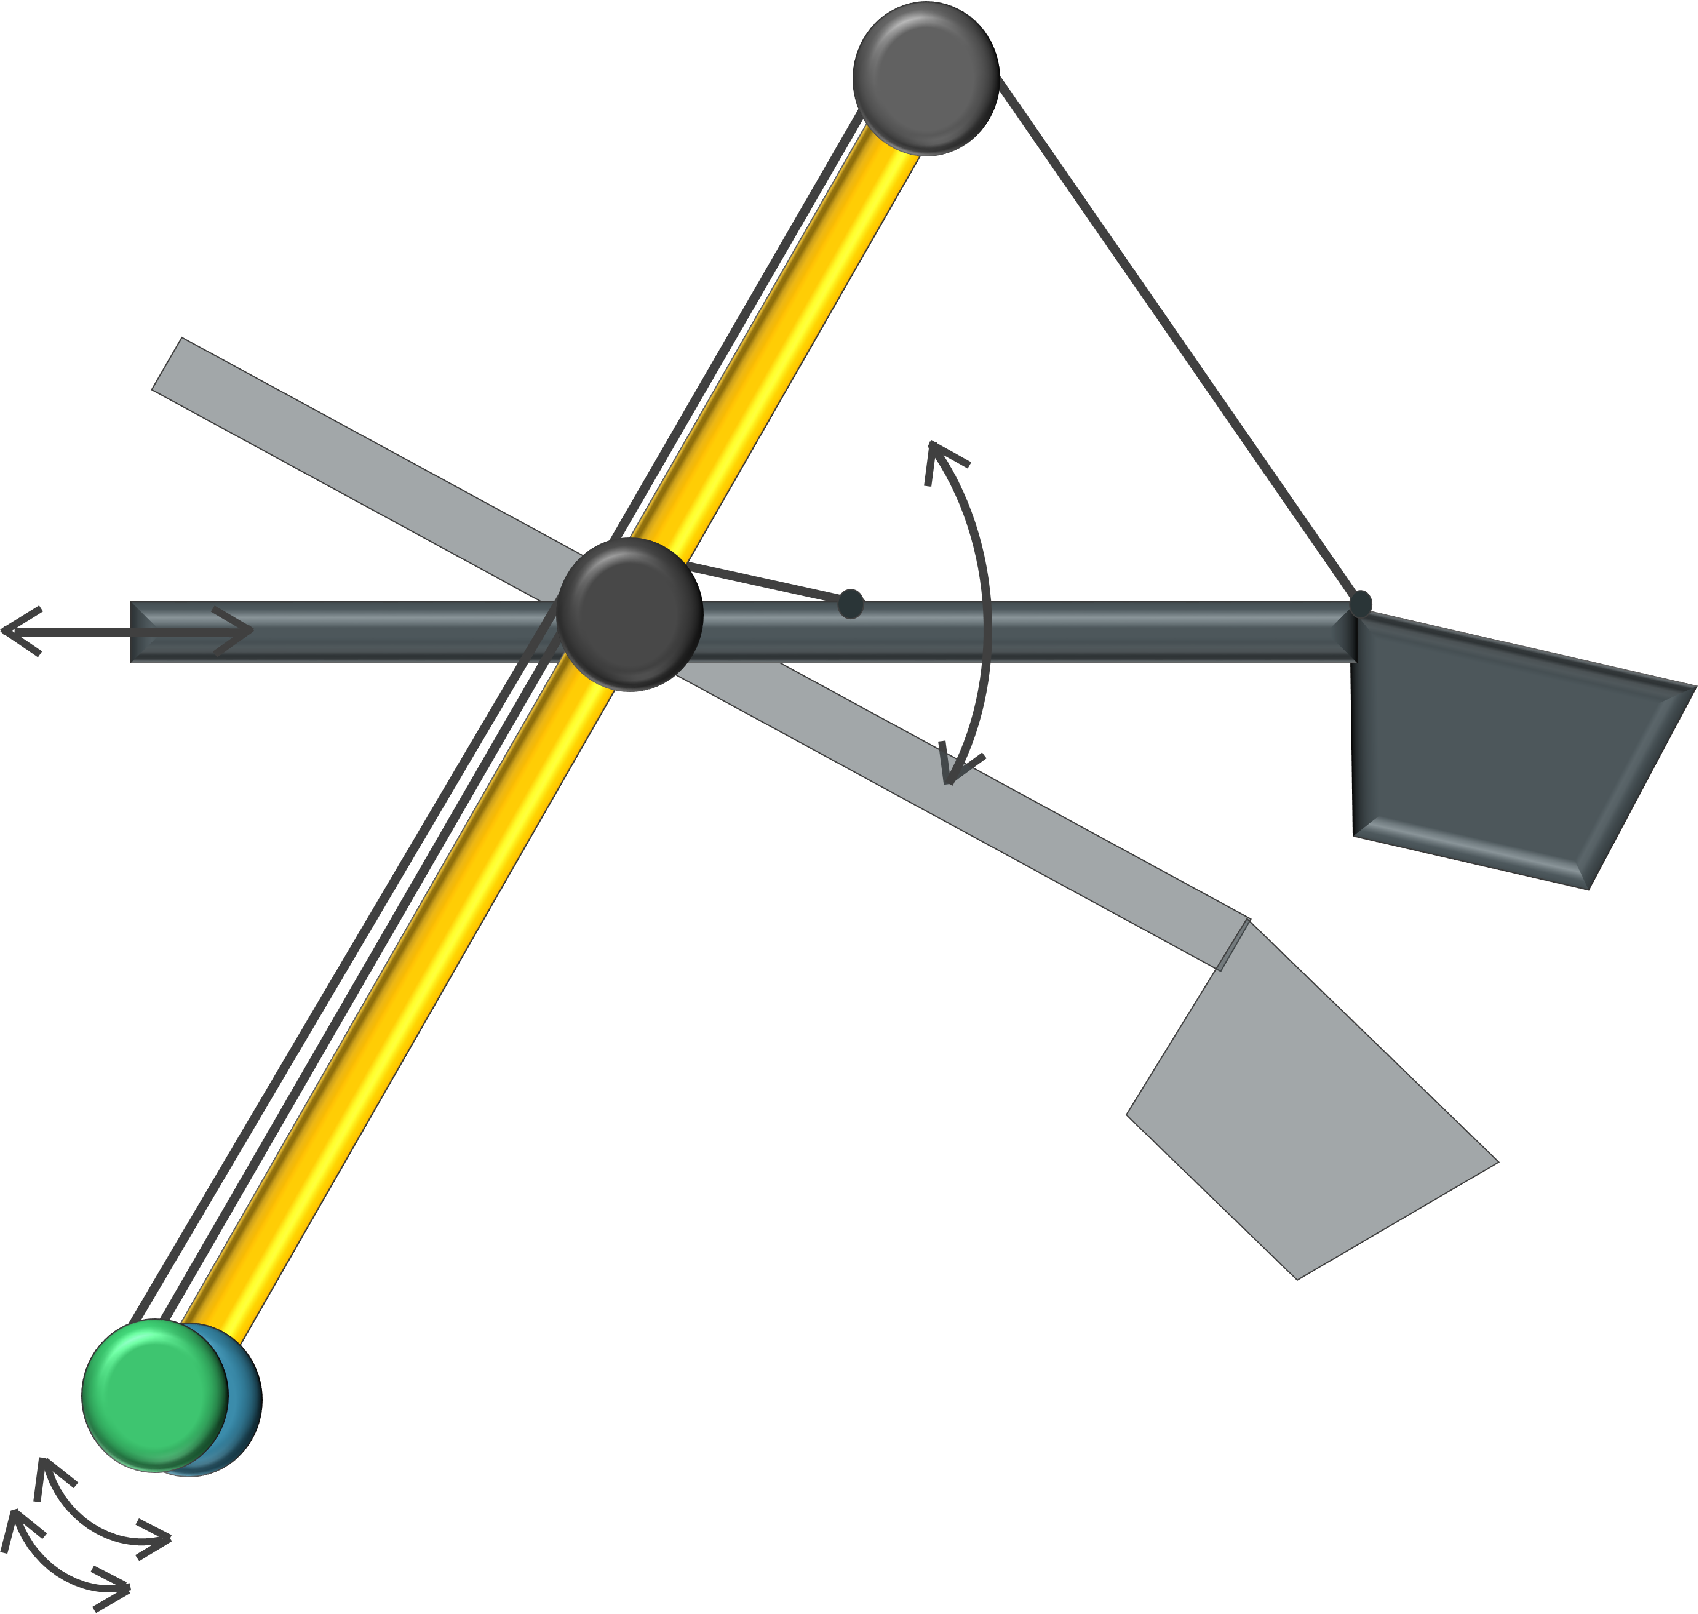
\includegraphics[width=0.4\linewidth]{img/Problem_2}
	\end{figure}
	\begin{itemize}
		\item{arm element fixed to base}
		\item{cannot be moved w.r.t. the base}
	\end{itemize}
\end{frame}

\begin{frame}
	\frametitle{Problem Setting}
	\begin{figure}[bth]
		\centering
		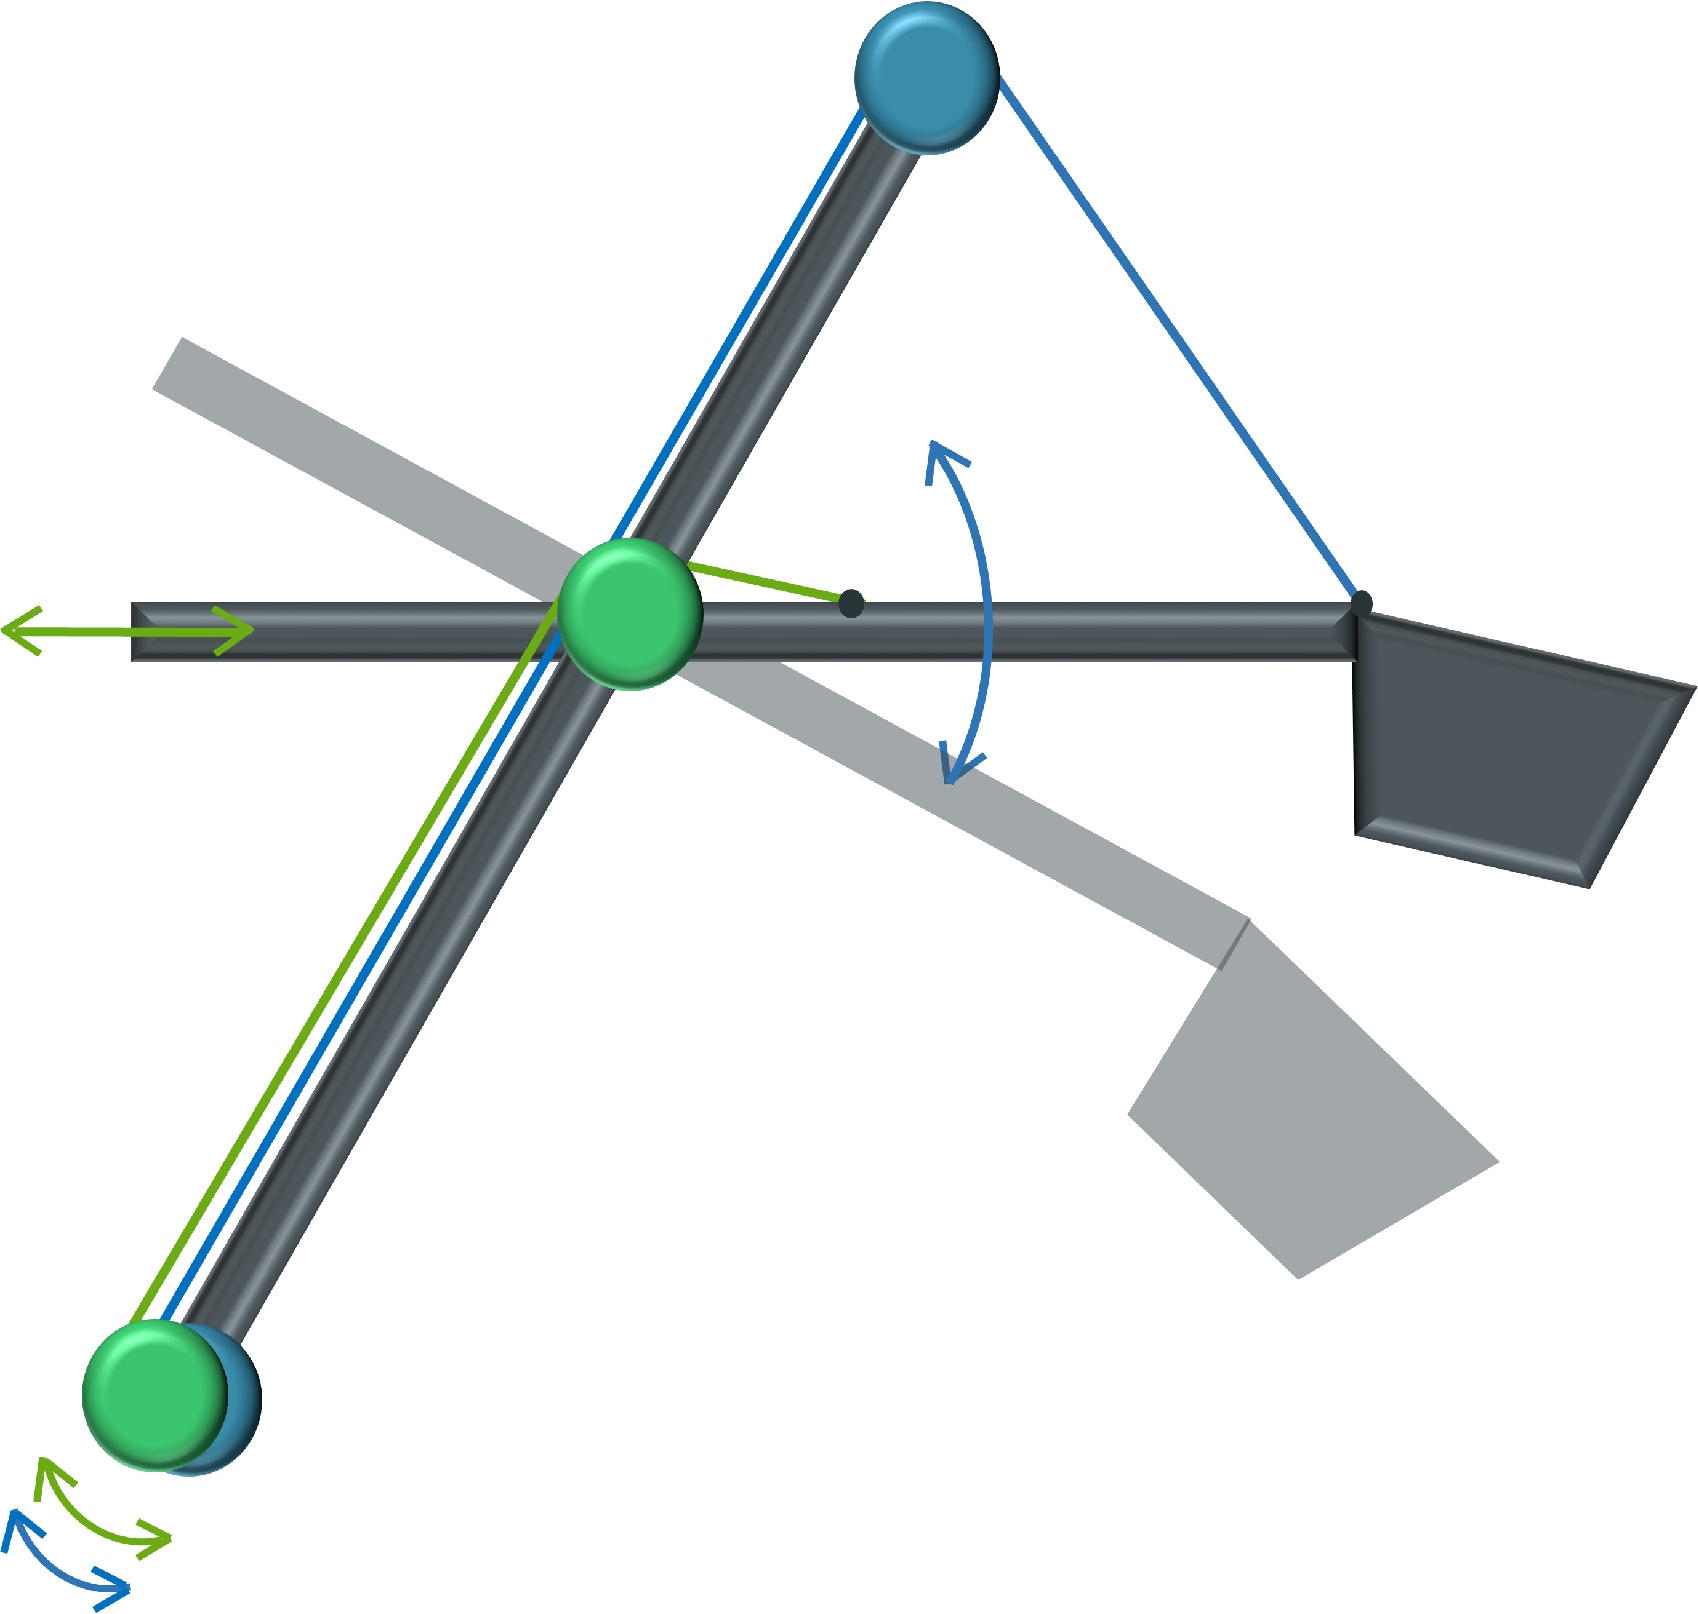
\includegraphics[width=0.4\linewidth]{img/Problem_3}
	\end{figure}
	\centering
	\begin{tabular}{ll}
		\textcolor[rgb]{0,0.69,0.32}{green} & shovel motion \textbf{back} and \textbf{forth} \\
		\textcolor[rgb]{0.18,0.46,0.71}{blue} & shovel motion \textbf{up} and \textbf{down} \\
	\end{tabular}
\end{frame}

\begin{frame}[c]
	\frametitle{Main Problems}
	\begin{enumerate}
		\item{Phyiscal Modelling}
			\begin{itemize}
				\item{modelling rope properties}
				\item{determining information needed for calibration of model}
			\end{itemize}
		\vspace{0.5cm}
		\item{Parameter Optimization}
			\begin{itemize}
				\item{optimizing parameters for a complex, unknown model (black box)}
			\end{itemize}
	\end{enumerate}
\end{frame}

\begin{frame}[c]
	\frametitle{Physical Modelling}
	Why?
	
	\vspace{0.5cm}
	
	\begin{columns}[t]
		\column{.3\linewidth}
			\centering
			\fbox{\parbox{\textwidth}{building an accurate model}}
		\column{.2\linewidth}
			\centering
			$\Rightarrow$
		\column{.3\linewidth}
			\centering
			\fbox{\parbox{\textwidth}{better visualization of control and motion}}
	\end{columns}
	
	\vspace{0.5cm}
	
	to consider:
	\begin{itemize}
		\item{friction in cable reels}
		\item{deformation of ropes}
	\end{itemize}
\end{frame}

\begin{frame}[c]
	\frametitle{Parameter Optimization}
	What are parameters?
	\begin{itemize}
		\item{friction coefficients}
		\item{mass}
		\item{inertia}
	\end{itemize}
	
	\vspace{0.5cm}
	
	Why?
	
	\vspace{0.5cm}
	
	\begin{columns}
		\column{.3\textwidth}
			\centering
			\fbox{\parbox{\textwidth}{accurate and realistic parameters}}
		\column{.2\textwidth}
			\centering
			$\Rightarrow$
		\column{.3\textwidth}
			\fbox{\parbox{\textwidth}{better prediction and planning of motion}}
	\end{columns}
\end{frame}


